\chapter{Implementation} % Main chapter title

\label{Chapter5}

\lhead{Chapter 5. \emph{Implementation}}

Each transformation is defined as a rewrite rule. It has a concrete syntax pattern which matches part of a parse-tree. The result is a concrete piece of syntax, using only constructs from the core syntax definition (i.e. ES 5).
The rewrite rules are exhaustively applied on the input parse-tree until no more rewrite rules match any sub-trees of the input. Application of rewrite rules to the parse-tree is done bottom-up because several rewrite rules (e.g. arrow function) demand their sub-terms to be transformed to guarantee successful completion.

\section{Basics}
To get a better understanding of the inner working of our rewrite rule system we discuss the implementation of the \lstinline$swap$ language extension (see section \ref{hygiene}). The language extension introduces a new statement 

\begin{lstlisting}[caption=Core syntax,language=rascal]
module core::Syntax

syntax Statement 
	= ...
	| ...
	...;
\end{lstlisting}

To extend the list of possible statements we create a new Rascal module that extends the core syntax definition and defines a new syntax rule for \textit{Statement} named \textit{swap}. With this new syntax rule our parser is able to correctly parse \lstinline$swap$ statements.

\begin{lstlisting}[caption=Swap statement syntax,language=rascal]
extend core::Syntax;

syntax Statement = swap: "swap" Id Id;
\end{lstlisting}

To desugar the new syntax construct to JavaScript code we overload the desugar function with a pattern match on 
\textit{Statement} to match the use of the \lstinline$swap$ statement and translate it to an IIFE in which we rebind both supplied identifiers to each other.

% \CAT{Keyword}{syntax} Statement = \CAT{Constant}{"swap"} Id Id;

\begin{rascal}
Statement desugar( (Statement)`\CAT{Keyword}{swap} \CAT{MetaVariable}{\textless{}Id x\textgreater{}} \CAT{MetaVariable} {\textless{}Id y\textgreater{}}` )
    = (Statement)
            `(\CAT{Keyword}{function}() \{{}
            	\CAT{Keyword}{var} tmp = x;
            	\CAT{MetaVariable}{\textless{}Id x\textgreater{}} = \CAT{MetaVariable}{\textless{}Id x\textgreater{}};
            	\CAT{MetaVariable}{\textless{}Id y\textgreater{}} = \CAT{MetaVariable}{\textless{}Id y\textgreater{}};
            \}{})();`;
\end{rascal}

A default desugar function for statements is defined which is the id function on a statement. To desugar an entire parse tree we only have to visit each node (bottom up) and invoke the desugar function for each statement that is found by the visitor.

\begin{lstlisting}[caption=Desugar visitor, language=rascal]
default Statement desugar( Statement s ) = s;

Source runDesugar( Source pt ) {
	return visit(pt) {
		case Statement s => desugar(s)
	}
}
\end{lstlisting}

\section{\projectname}
In \textit{\projectname} we implement a large subset of ES6 features as language extensions on top of a core syntax describing ES5. Here we discuss several parts of interest from our implementation. Everything with the exception of let-const is based on the simple example described in the previous section. 

\subsection{Visitor}
The visitor from our basic example is almost identical in \projectname. Differences are we also match on expressions, functions, and the source node (root node) this final match can be used by transformations that are performed global-to-local or global-to-global. If we have multiple language extensions performing a global-to-local or global-to-global transformation or if a language extension's transformation introduces a language construct that should be desugared either by itself or another language extension, one pass over the parse tree is not enough. For extensions with these kind of transformations we need to revisit the tree until no more changes are applied by desugar functions. The final desugar visitor is as follows, where \textit{solve} will ensure we revisit the tree until no more desugarings are performed:

\begin{lstlisting}[caption=Final desugar visitor, language=rascal]
Source runDesugar( Source pt ) {
	return solve(pt) {
		pt = visit(pt) {
			case Source src => desugar(src)
			case Function f => desugar(f)
			case Statement s => desugar(s)
			case Expression e => desugar(e)
		}
	}
}
\end{lstlisting}

An example of a language extension that relies on a global-to-local transformation is the arrow function. Arrow function's that reside directly in the global scope, not inside another function, are desugared differently. See appendix \ref{arrow}

\subsection{Introducing bindings}
Some language extensions need to introduce new bindings in the target program to work properly. There are multiple ways for a transformation to introduce bindings in JavaScript. When a transformation is performed on an expression an IIFE can be used to introduce new bindings only accesible in the scope of this expression.

\begin{minipage}{0.45\linewidth}
\begin{lstlisting}
<Expression e>
\end{lstlisting}
\end{minipage}
\hfill
\begin{minipage}{0.45\linewidth}
\begin{lstlisting}
(function(x, y, ...) {
	return <Expression e>;
})(xd, yd, ...)
\end{lstlisting}
\end{minipage}

When a transformation is performed on a statement a block statement can be used in combination with variables declared through the \textit{let} declarator, to introduce variables only accessible in the scope of the statement:

\begin{minipage}{0.45\linewidth}
\begin{lstlisting}
<Statement s>
\end{lstlisting}
\end{minipage}
\hfill
\begin{minipage}{0.45\linewidth}
\begin{lstlisting}
{
	let x = xd,
		y = yd
		...;
	<Statement s>
}
\end{lstlisting}
\end{minipage}

In the case of a statement an IIFE can not be used to introduce new bindings because the control-flow of the target program would break if the desugared statement contains a control-flow construct (e.g. it returns a value), now this value is returned in our IIFE and not its lexical enclosing function.

\subsection{Combined language extensions} \label{par:combined-extensions}
Language extensions can depend upon other language extensions to work correctly, this dependency makes a collection of language extensions less modular because the depended extension always needs to be used in combination with it's dependency. It would be preferable if the two extensions could be used in separation where functionality which relies on both extensions working together is only enabled in a situation where the two language extensions are used.

An example of such overlapping functionality in the ES 6 specification is that of destructuring assignment (see appendix \ref{destructuring}) inside for-of loops (see appendix \ref{for-of}).

\begin{lstlisting}
for(var [a,b] of [ [1,2], [3,4] ]) {
	// ... do something with a and b
}
\end{lstlisting}

The for-of loop needs a dependency on the destructuring assignment syntax definition, to be able to create the statement syntax to allow an assignment pattern (i.e. either an array or object destructuring) inside the for-of loop:

\begin{lstlisting}[language=rascal]
syntax Statement
	= "for" "(" "var" AssignmentPattern "of" Expression ")" Statement;
\end{lstlisting}

Shared language extensions need to have a non-terminal defined in the base-language which can be extended in both language extensions. In case of the for-of loop we can introduce a new non-terminal \textit{ForBinding} which can be extended in the destructuring assignment language extension.

\begin{lstlisting}[language=rascal]
// Core syntax definition
syntax ForBinding
	= Id;

// For-of loop language extension
syntax Statement
	= "for" "(" "var" ForBinding "of" Expression ")" Statement;

// Destructuring language extension
syntax ForBinding
	= AssignmentPattern;
\end{lstlisting}

Designing language extensions in this way makes the entire suite of language extensions more modular, because we remove unnecessary dependencies between extensions. We can combine language extensions that depend on each other for full functionality. Or use them separately to get only their independent functionality.

\subsection{Variable capture}
In section \ref{hygiene} we have described the problem of variable capture in the context of program transformations. 
Here we discuss the code reused to solve variable capture in \projectname, the algorithm reused is name \textit{\vfix}. The algorithm relies on a binding graph to identify variable capture, and uses string origins~\cite{Inostroza2014} to distinguish between synthesized identifiers (i.e. those identifiers introduced by the transformation) and identifiers originating from the source program.

\textit{\vfix} analyses the \textit{name graph} of source and target program to identify variable capture. The name graph contains nodes for all identifiers in the program, a directed edge indicates a reference to a declaration. Because our source and target language are both JavaScript and thus have the same binding mechanism, we only generate the name graph for our target program. In the graph a distinction is made between synthesized and user bindings. To identify whether a binding originates from the source program or was synthesized during transformation, the \textit{\vfix} algorithm uses string origins~\cite{Inostroza2014}.

In figure \ref{fig:name-graph} we use the target program from our \lstinline$swap$ language extension (see section \ref{hygiene}) to illustrate how these name graphs are constructed, and how \textit{\vfix} identifies variable capture. Each node contains a line number and the identifier it resembles from that line, a directed edge is a reference to a declaration. Nodes with a white background originate from the source program, nodes with a dark background are synthesized during transformation. Line numbers from synthesized identifiers are appended with a tick.

\begin{figure}[h]
\centering
\begin{minipage}{0.25\linewidth}
\begin{lstlisting}
	var x = 0,
		tmp = 1;

	(function() {
		var tmp = x;
		x = tmp;
		tmp = tmp;
	})();
\end{lstlisting}
\end{minipage}
\hfill
\begin{minipage}{0.65\linewidth}
\begin{tikzpicture}[
source/.style={circle, draw=black, fill=white, very thick, minimum size=10mm},
synthesized/.style={circle, draw=black, fill=gray!60, very thick, minimum size=10mm}
]
\node[source](x_dec){1:x};
\node[source](tmp_dec)[right=of x_dec]{2:t};
\node[synthesized](tmp_dec_2)[right=of tmp_dec]{5':t};

\node[source](x_ref)[below=of x_dec,xshift=7mm]{5:x};
\node[source](x_ref_2)[below=of x_dec,xshift=-7mm]{6:x};
\node[source](tmp_ref)[below=of tmp_dec_2,xshift=-7mm]{6:t};
\node[synthesized](tmp_ref_2)[below=of tmp_dec_2,xshift=7mm]{7':t};

\node[source](tmp_ref_3)[below=of tmp_dec]{7:t};

\draw[->] (x_ref.north) -- (x_dec.south);
\draw[->] (x_ref_2.north) -- (x_dec.south);
\draw[->] (tmp_ref.north) -- (tmp_dec_2.south);
\draw[->] (tmp_ref_2.north) -- (tmp_dec_2.south);
\draw[->] (tmp_ref_3.north) -- (tmp_dec_2.south);
\end{tikzpicture}
\end{minipage}

\caption{Target program generated by swap language extension and corresponding name graph} \label{fig:name-graph}
\end{figure}

Node \textit{7:t} and \textit{6:t} originate from the source program but reference a synthesized declaration. Node \textit{5:t} shadows the original declaration \textit{2:t}. \textit{\vfix} adds node \textit{5:t} to the list of declarations to be renamed. After the entire name graph is analyzed/generated all declarations from this list are rebound under free names (i.e. names not yet bound in the target program). Since \textit{7:t} and \textit{6:t} are not correct references of \textit{5:t} they are not renamed. The resulting name graph and target program are presented in figure \ref{fig:name-graph-fixed}

\begin{figure}[h]
\centering
\begin{minipage}{0.25\linewidth}
\begin{lstlisting}
	var x = 0,
		tmp = 1;

	(function() {
		var tmp$0 = x;
		x = tmp;
		tmp = tmp$0;
	})();
\end{lstlisting}
\end{minipage}
\hfill
\begin{minipage}{0.65\linewidth}
\begin{tikzpicture}[
source/.style={circle, draw=black, fill=white, very thick, minimum size=10mm},
synthesized/.style={circle, draw=black, fill=gray!60, very thick, minimum size=10mm}
]
\node[source](x_dec){1:x};
\node[source](tmp_dec)[right=of x_dec,xshift=7mm]{2:t};
\node[synthesized](tmp_dec_2)[right=of tmp_dec]{5':t'};

\node[source](x_ref)[below=of x_dec,xshift=7mm]{5:x};
\node[source](x_ref_2)[below=of x_dec,xshift=-7mm]{6:x};
\node[source](tmp_ref)[below=of tmp_dec,xshift=7mm]{6:t};
\node[synthesized](tmp_ref_2)[below=of tmp_dec_2]{7':t'};

\node[source](tmp_ref_3)[below=of tmp_dec,xshift=-7mm]{7:t};

\draw[->] (x_ref.north) -- (x_dec.south);
\draw[->] (x_ref_2.north) -- (x_dec.south);
\draw[->] (tmp_ref.north) -- (tmp_dec.south);
\draw[->] (tmp_ref_2.north) -- (tmp_dec_2.south);
\draw[->] (tmp_ref_3.north) -- (tmp_dec.south);
\end{tikzpicture}
\end{minipage}

\caption{Target program and name graph after \textit{\vfix} algorithm} \label{fig:name-graph-fixed}
\end{figure}

\textit{\vfix} does apply a \textit{"closed-world assumption to infer that all unbound variables are indeed free, and thus can be renamed at will."}~\cite{Erdweg2014}. This means that global variables defined by the user (or a third-party library) that are included within the same run-time as our target program, could possibly be shadowed by the renamed bindings. However there is no way for \textit{\vfix} to know what bindings will be taken by other bindings than those bound in the source program.

A second form of variable capture is introduced when the user shadows a global variable on which a target program relies. \textit{\vfix} is also able to solve this form of variable capture, to illustrate this we use the example of the \lstinline$log$ language extensions. The name-graph for the target program of our example (see section \ref{hygiene}) shows a reference from an identifier introduced by our transformation to a source binding (see figure \ref{fig:vfix2}).

\begin{figure}[h]
\centering
\begin{minipage}{0.65\linewidth}
\begin{lstlisting}
	var console = <Expression e>;
	console.log("message");
	console;
\end{lstlisting}
\end{minipage}
\hfill
\begin{minipage}{0.25\linewidth}
\begin{tikzpicture}[
source/.style={circle, draw=black, fill=white, very thick, minimum size=10mm},
synthesized/.style={circle, draw=black, fill=gray!60, very thick, minimum size=10mm}
]
\node[source](console_dec){1:c};

\node[synthesized](console_ref)[below=of console_dec,xshift=-7mm]{2:c};
\node[source](console_ref_2)[below=of console_dec,xshift=7mm]{3:c};

\draw[->] (console_ref.north) -- (console_dec.south);
\draw[->] (console_ref_2.north) -- (console_dec.south);
\end{tikzpicture}
\end{minipage}
\caption{Target program generated by log language extension and corresponding name-graph} \label{fig:vfix2}
\end{figure}

This reference is identified as variable capture and declaration \lstinline$console$ is marked to be renamed (see figure \ref{fig:vfix2}. 

\begin{figure}[h]
\centering
\begin{minipage}{0.65\linewidth}
\begin{lstlisting}
	var console$0 = <Expression e>;
	console.log("message");
	console$0;
\end{lstlisting}
\end{minipage}
\hfill
\begin{minipage}{0.25\linewidth}
\begin{tikzpicture}[
source/.style={circle, draw=black, fill=white, very thick, minimum size=10mm},
synthesized/.style={circle, draw=black, fill=gray!60, very thick, minimum size=10mm}
]
\node[source](console_dec){1:c};

\node[synthesized](console_ref)[below=of console_dec,xshift=-7mm]{2:c};
\node[source](console_ref_2)[below=of console_dec,xshift=7mm]{3:c};

\draw[->] (console_ref_2.north) -- (console_dec.south);
\end{tikzpicture}
\end{minipage}
\caption{Target program and name-graph after application of \textit{\vfix} algorithm} \label{fig:vfix2_fixed}
\end{figure}

\subsection{Block binding}
To desugar the new block binding introduced in ES6 (see appendix \ref{let-const}) there are two approaches. First, replace all block binding by a \textit{try catch} block where we throw the binding inside of try and catch the binding in the catch block.

\begin{minipage}{0.45\linewidth}
\begin{lstlisting}
let x = 0;
... statements
\end{lstlisting}
\end{minipage}
\hfill
\begin{minipage}{0.45\linewidth}
\begin{lstlisting}
try {
	throw 0;
} catch(x) {
	... statements
}
\end{lstlisting}
\end{minipage}

The problem with this implementation is that \textit{try catch} blocks can not be optimized by the interpreter and thus the performance of transformed code could be much worse than that of the source program. Second, the block binding could be achieved through the renaming of bindings to avoid reference of \textit{let} defined bindings outside of their block scope.

\begin{minipage}{0.45\linewidth}
\begin{lstlisting}
{
	let x = 0;
	x;
}
x;
\end{lstlisting}
\end{minipage}
\hfill
\begin{minipage}{0.45\linewidth}
\begin{lstlisting}
{
	var x_0 = 0;
	x_0;
}
x;
\end{lstlisting}
\end{minipage}

To resolve the naming needed for the emulation of block scope in ES5 we also use a \textit{name-graph} as described in the previous section. To identify illegal references in the name graph we compare a name graph with block binding against a name graph without block binding, the two graphs for the example are depicted below:

\begin{figure}
\begin{subfigure}{.45\textwidth}
\centering
\resizebox{0.4\linewidth}{!}{
\begin{tikzpicture}[
source/.style={circle, draw=black, fill=white, very thick, minimum size=10mm},
synthesized/.style={circle, draw=black, fill=gray!60, very thick, minimum size=10mm}
]
\node[synthesized](x_dec)[align=center]{2:x};

\node[source](x_ref)[below=of x_dec,xshift=-7mm]{3:x};
\node[source](x_ref_2)[below=of x_dec,xshift=7mm]{5:x};

\draw[->] (x_ref.north) -- (x_dec.south);
\end{tikzpicture}
}
\subcaption{Name graph (block scope binding)}
\end{subfigure}
\hfill
\begin{subfigure}{.45\textwidth}
\centering
\resizebox{0.4\linewidth}{!}{
\begin{tikzpicture}[
source/.style={circle, draw=black, fill=white, very thick, minimum size=10mm},
synthesized/.style={circle, draw=black, fill=gray!60, very thick, minimum size=10mm}
]
\node[synthesized](x_dec){2:x};

\node[source](x_ref)[below=of x_dec,xshift=-7mm]{3:x};
\node[source](x_ref_2)[below=of x_dec,xshift=7mm]{5:x};

\draw[->] (x_ref.north) -- (x_dec.south);
\draw[->] (x_ref_2.north) -- (x_dec.south);
\end{tikzpicture}
}
\subcaption{Name graph (function scope binding)}
\end{subfigure}
\end{figure}

The first name graph is that created using a block binding mechanism where \textit{const} and \textit{let} declarations are block bound. In the second name graph all declarations are bound in their lexical enclosing function's scope. Now we identify the reference from \textit{5:x} to the declaration \textit{2:x} as illegal, because it exists in our function scoped name graph but does not occur in the block bound name graph. Declaration \textit{2:x} is marked to be renamed. After the entire name graph is build and all illegal references are identified, all declarations and their references according to the block bound name graph are renamed.

\paragraph{implementation}
For the implementation of the block binding resolver we use a special type of scope graph, consisting of three types of nodes. First, a root node created for the root (or global) scope of an input parse tree. This node contains an environment consisting of names with the location of their declaration. Second, each function scope is identified by a closure node. This node consists of an \lstinline$Env$ containing all function scoped definitions (i.e. declarations of functions or using \lstinline$var$ declarator). It also contains a \lstinline$LEnv$ which is the name-graph created where all bindings are function scoped (i.e. also declarations using \lstinline$let$ or \lstinline$const$ declarators). Third, a node block is created for each block of statements, containing all block-scoped declarations in an environment.

\begin{lstlisting}[caption=Data structure for scope graph,language=rascal]
alias LEnv = lrel[str name, loc def];
alias Env = map[str name,loc def];

data Scope 
	= block( Env environment, Scope parent )
	| closure( Env environment, LEnv closureEnvironment, Scope parent )
	| root( Env environment );
\end{lstlisting}

A resolver visits the parse-tree while building a scope trees for the current path. All declaration in a function's scope are hoisted, because these declarations can be referenced throughout the entire lexical scope of the function, even before their actual declaration. Usage of an identifier by reference are resolved through a function named \lstinline$lookup$:

\begin{lstlisting}[language=rascal]
set[loc] lookup(str name, loc use, Scope scope);
\end{lstlisting}

This function visits the scope tree (top-down, the root of the tree is the current scope). For block and root nodes the location of declaration of the binding is returned if it is present in the environment of that scope. If no declaration is found in block scopes and we visit a closure node we first identify whether any \textit{illegal} references are possible to declarations in other block scopes not accesible from our scope. Then we lookup whether a declaration exists in the current closure and return this declaration if it exists.

To detect illegal redeclarations a function name \lstinline$declare$ is called on each declaration. It checks whether the name is already declared in the current block-scope, in this case it sets an error message. If the binding is not yet declared in the block-scope it checks whether it is set in any other block-scopes of the current closure, in this case the declaration is marked for renaming.

\begin{lstlisting}[language=rascal]
bool declare(loc decl, str name, loc def, Scope scope);
\end{lstlisting}

\subsection{IDE integration}
Because the features described in the previous two sections need name graph analysis we can perform some static analysis on these graphs and integrate the resulting data with the IDE. First, the name graph gives us information of all references in the source file, with this information we create hyperlinks from references to declarations. Second, we can also identify a reference to an undefined binding and mark this reference with an error inside the IDE. Finally, bindings created by let (or const) are not allowed to be re-declared in the same scope, illegal redeclarations can be identified and marked with an error in the IDE.

\begin{figure}
\centering

\begin{subfigure}{.49\textwidth}
	\centering
	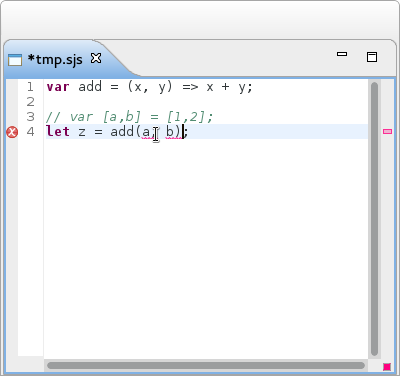
\includegraphics[width=\textwidth]{undeclared.png}
	\subcaption{Reference of undeclared bindings}
\end{subfigure}\hfill%
\begin{subfigure}{.49\textwidth}
	\centering	
	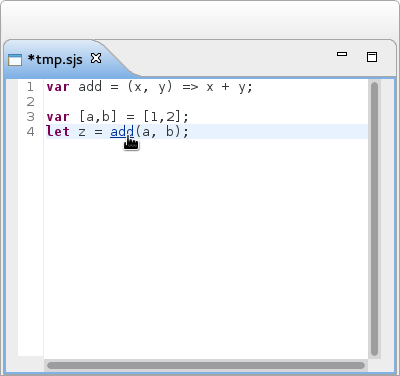
\includegraphics[width=\textwidth]{declared-at.png}
	\subcaption{Declared at hyperlink}
\end{subfigure}

\caption{IDE support}
\end{figure}